%% signed-decomposition.tex — Signed Decomposition of the Regression Structure via Linear JEPA Training
%% Compile: pdflatex signed-decomposition && bibtex signed-decomposition && pdflatex signed-decomposition && pdflatex signed-decomposition

\documentclass[reqno,11pt]{amsart}

%% ── Encoding & fonts ─────────────────────────────────────────────────────────
\usepackage[utf8]{inputenc}
\usepackage[T1]{fontenc}
\usepackage{microtype}

%% ── Mathematics ──────────────────────────────────────────────────────────────
\usepackage{amsmath,amssymb,amsthm}
\usepackage{mathtools}
\usepackage{array}

%% ── Figures ──────────────────────────────────────────────────────────────────
\usepackage{graphicx}
\usepackage{subcaption}
\usepackage{tikz}

%% ── Bibliography ─────────────────────────────────────────────────────────────
\usepackage[numbers,sort&compress]{natbib}

%% ── Hyperlinks ───────────────────────────────────────────────────────────────
\usepackage[dvipsnames,svgnames,x11names]{xcolor}
\usepackage[colorlinks=true,
            linkcolor=RoyalBlue4,
            citecolor=RoyalBlue4,
            urlcolor=NavyBlue]{hyperref}
\usepackage{url}
\usepackage{xurl}

%% ── Page geometry ────────────────────────────────────────────────────────────
\usepackage[top=1in,bottom=1in,left=1in,right=1in]{geometry}

%% ── Enumitem for tighter lists ───────────────────────────────────────────────
\usepackage{enumitem}

%% ── Bold run-in \paragraph headings ─────────────────────────────────────────
\makeatletter
\renewcommand\paragraph{%
  \@startsection{paragraph}{4}{\z@}%
    {1.5ex \@plus 0.5ex \@minus 0.2ex}%
    {-0.6em}%
    {\normalfont\normalsize\bfseries}}
\makeatother

%% ─────────────────────────────────────────────────────────────────────────────
%%  MACROS
%% ─────────────────────────────────────────────────────────────────────────────

\newcommand{\RR}{\mathbb{R}}
\newcommand{\NN}{\mathbb{N}}
\newcommand{\EE}{\mathbb{E}}
\newcommand{\PP}{\mathbb{P}}
\DeclareMathOperator{\tr}{tr}
\DeclareMathOperator{\sign}{sign}
\DeclareMathOperator*{\argmin}{arg\,min}

\newcommand{\lean}[1]{\textup{\small\nolinkurl{#1}}}

\newcommand{\Wbar}{\bar{W}}
\newcommand{\Sxx}{\Sigma^{xx}}
\newcommand{\Syx}{\Sigma^{yx}}
\newcommand{\eps}{\varepsilon}
\newcommand{\rhostar}{\rho_r^*}
\newcommand{\lamstar}{\lambda_r^*}
\newcommand{\sigmar}{\sigma_r}
\newcommand{\rhohat}{\hat{\rho}_r}
\newcommand{\lamhat}{\hat{\lambda}_r}
\newcommand{\muhat}{\hat{\mu}_r}
\newcommand{\rhoplateau}{\rhohat^{\mathrm{plateau}}}

%% ─────────────────────────────────────────────────────────────────────────────
%%  THEOREM ENVIRONMENTS
%% ─────────────────────────────────────────────────────────────────────────────

\theoremstyle{plain}
\newtheorem{theorem}{Theorem}[section]
\newtheorem{lemma}[theorem]{Lemma}
\newtheorem{proposition}[theorem]{Proposition}
\newtheorem{corollary}[theorem]{Corollary}

\theoremstyle{definition}
\newtheorem{definition}[theorem]{Definition}
\newtheorem{assumption}[theorem]{Assumption}

\theoremstyle{remark}
\newtheorem{remark}[theorem]{Remark}

%% ─────────────────────────────────────────────────────────────────────────────
%%  DOCUMENT
%% ─────────────────────────────────────────────────────────────────────────────

\begin{document}

\title[Signed Decomposition via Linear JEPA Training]
      {Signed Decomposition of the Regression Structure\\
       via Linear JEPA Training:\\
       An Algorithm, Empirical Validation, and a Machine-Checked Proof}

\author{Goh Cheng Arn David}
\address{Department of Computer Science, University of Toronto}
\email{daveed@cs.toronto.edu}
\date{May 2026}

\begin{abstract}
A depth-$L$ linear Joint Embedding Predictive Architecture (JEPA) encoder, during
training, assigns weight to each
feature indicative of its relevance or usefulness to the prediction
task. These dynamics are exactly solvable.
We ask if the signed regression spectrum $\{\rhostar\}$ of the pencil
$(\Syx, \Sxx)$ can be recovered from the trajectories of these weights
alone, without knowing the population covariances of the features.
We present an estimator whose form depends on the sign of each
feature's regression coefficient $\rhostar$, which is itself read off
the trajectory's asymptotic shape.
On the positive branch, the plateau value recovers $\rhostar$ at rate
$O(\eps^{1/L}|\log\eps|)$, given only the eigenbasis.
On the negative branch, the decay rate recovers the projected
covariance at the same order, while the sample covariance recovers the
quadratic form of the feature's eigenvector.
The construction is packaged as the algorithm \textsc{PlateauRecover}.
It is verified in Lean~4, with zero \texttt{sorry} and two named axioms.
The ordering theorem of \citet{Goh2026ordering} falls out as a
corollary of the positive-branch trichotomy.
\end{abstract}

\maketitle


%% ─────────────────────────────────────────────────────────────────────────────
%%  SECTIONS
%% ─────────────────────────────────────────────────────────────────────────────

\section{Introduction}
\label{sec:intro}

Joint Embedding Predictive Architecture (JEPA) has been the subject of much active development. It
predicts in latent/embedding space rather than reconstructing pixels, discarding
irrelevant or unpredictable detail to focus on high-level structure. However, almost nothing is known rigorously about what its training dynamics do to the
underlying data structure.

We find that JEPA training dynamics themselves partition every feature direction by its true
predictive relationship to the target. We prove that in the linear JEPA
context, we get signed, per-feature regression, decodable from the
encoder's internal weight trajectory. We have an explicit signed
estimator computable from the trajectory alone, and an easy to deploy
algorithm we call \textsc{PlateauRecover} (code provided). Concretely:
the sign of $\rhostar$ is always recoverable from the trajectory
$\sigmar(t)$ alone, and on the positive branch so is its magnitude
(given only the eigenbasis, no further population-covariance input
needed) at rate $O(\eps^{1/L}|\log\eps|)$, a corollary of the
results in \S\ref{sec:estimating-spectrum}
(Theorem~\ref{thm:headline-formal}).

\label{ssec:positioning}
In the linear case, everything we recover here is something OLS (or
other gradient-descent methods) could already give us. We care about
it because it is a critical stepping stone to the non-linear regime of
representation learning on unlabeled data. There, there may be no
clean $y$, no fixed $\Sigma^{xx}$-type inner product, and no
normal-equations solver to fall back on. In particular, the
LeWorldModel architecture of \citet{Maes2026LeWM} is exactly such a
case. There, the training trajectory is the only handle on the
underlying regression structure: $\{\rhostar\}$ can be read off a
JEPA training trajectory without ever forming $\Sigma^{xx}, \Sigma^{yx}$.

\subsection*{Notation}

We fix notation for the covariances and the regression spectrum they define.
For data pairs $(x,y)\in\RR^d\times\RR^d$, write
$\Sigma^{xx} := \EE[xx^\top] \succ 0$ for the input covariance and
$\Sigma^{yx} := \EE[yx^\top]$ for the target-input cross-covariance.
The regression structure we recover throughout the paper is read off the
generalized eigenproblem
\[
\Sigma^{yx} v_r^* = \rho_r^* \Sigma^{xx} v_r^*.
\]
Unlike an ordinary eigenvector, $v_r^*$ is fixed only up to an
arbitrary rescaling. The generalized eigenvalue $\rho_r^*$ itself is
untouched by this rescaling, since it is a property of the
eigen-direction rather than of any particular representative $v_r^*$.
What does move is the $\Sigma^{xx}$-quadratic form
$\mu_r := v_r^*\cdot\Sigma^{xx}v_r^*$ of $v_r^*$ (guaranteed $>0$ since
$\Sigma^{xx}\succ0$), and with it the projected covariance
$\lambda_r^* := \rho_r^*\mu_r$. This invariance makes $\rho_r^*$ the
signed regression coefficient the rest of the paper tracks. The
collection $\{\rho_r^*\}_{r=1}^d$ (one signed scalar per feature
direction) is the ``regression spectrum'' of the pencil
$(\Sigma^{yx}, \Sigma^{xx})$ we are after. We package the triple
$(\rhostar, \mu_r, v_r^*)$ into a single labeled object that fixes this
scale-dependence once and for all:

\begin{definition}[Signed generalised eigenbasis]
\label{def:eigenbasis}
A \emph{signed generalised eigenbasis} for the pencil $(\Syx, \Sxx)$ is
a tuple $\{(\rhostar, \mu_r, v_r^*)\}_{r=1}^{d}$ with
$\rhostar \in \RR$, $v_r^* \in \RR^d \setminus \{0\}$,
$v_r^* \cdot \Sxx v_s^* = 0$ for $r \neq s$, and
\begin{equation}
\label{eq:gen-eigenpair}
\Syx v_r^* = \rhostar \Sxx v_r^*,
\qquad
\mu_r := v_r^* \cdot \Sxx v_r^*,
\qquad
\lamstar := \rhostar \mu_r.
\end{equation}
$\mu_r > 0$ is \emph{not} normalised to $1$. It is the free
$\Sxx$-quadratic form of the (arbitrarily scaled) eigenvector $v_r^*$,
matching \lean{Basic.SignedGenEigenpair.hmu_def}. Rescaling $v_r^*$
rescales $\mu_r$ and $\lamstar$ together while leaving
$\rhostar = \lamstar/\mu_r$ fixed, so $(\lamstar, \mu_r)$ is only
meaningful jointly, given a fixed scale for $v_r^*$. $\rhostar$ itself
is the scale-invariant quantity this paper recovers.
\end{definition}

\label{ssec:linear-jepa}
We now describe the model whose training we study: fix dimension $d$
and depth $L\ge2$ throughout (equal input/output dimension; the
rectangular case is left to future work). A depth-$L$ linear JEPA
factors its encoder as $\bar W = W_L\cdots W_1$,
each factor $W_a\in\RR^{d\times d}$ kept separate (never collapsed into
one matrix), plus a single unfactored predictor $V\in\RR^{d\times d}$.
This model trains to minimize the squared reconstruction error
\[
\mathcal{L}(\bar W, V) \;=\; \tfrac{1}{2}\,\EE\!\left[\big\|y - V \bar W x\big\|_2^2\right].
\]

This same eigenbasis is where the resulting training trajectory lives:
under aligned balanced initialisation, the encoder's weight matrix
$\Wbar(t)$ stays diagonal in it for all $t \ge 0$. Its diagonal entry
$\sigmar(t) := v_r^{*\top}\Wbar(t)v_r^*$ is the amplitude of feature
$r$ at time $t$. It obeys a Bernoulli-type ODE decoupled across
features at leading order, stated precisely as
Proposition~\ref{prop:diagonal-ode} in \S\ref{sec:diagonal-ode}
(equation~\eqref{eq:diagonal-ode}). Recovering $\{\rhostar\}$ means
understanding what training under this loss does to $\bar W$ and $V$
over time. This is where population gradient flow comes in.

\subsection*{Assumptions}
\label{ssec:assumptions-intro}

We work throughout under the following standing assumptions.

\begin{enumerate}[label=(A\arabic*),ref=A\arabic*,leftmargin=2.5em,itemsep=4pt]

\item \label{ass:population-flow}
\textbf{Exact population gradient flow.} Training proceeds under
\begin{equation}
\label{eq:jepa-flow}
\dot{\Wbar} = -\nabla_{\Wbar} \mathcal{L}
\ \ \text{(shorthand for the preconditioned flow of Lemma~\ref{lem:grad-flow})},
\qquad
\dot{V} = -\nabla_{V} \mathcal{L}.
\end{equation}
This is the theoretical idealisation; Algorithm~\ref{alg:plateau-recover}
(\S\ref{sec:algorithm}) instead runs discretised SGD on finite samples.

\item \label{ass:aligned-init}
\textbf{Aligned balanced initialisation.} We restrict throughout to
initialisation at scale $\eps\in(0,1)$:
\begin{equation}
\label{eq:init}
\bar W(0) = \eps \cdot U_x^\top U_x,
\qquad
V(0) = \eps \cdot U_y U_x^\top,
\end{equation}
where $U_x$ is the orthogonal basis of generalised eigenvectors of the
pencil $(\Sigma^{yx}, \Sigma^{xx})$ and $U_y$ its $\Sigma^{xx}$-orthonormal
image under $\Sigma^{yx}$ (Definition~\ref{def:eigenbasis}). The
balance condition is preserved under \eqref{eq:jepa-flow}
\citep{Saxe2014,Arora2018}. Exact alignment cannot hold in practice ---
the eigenbasis is unknown at initialisation; every identifiability result
here is stated under \eqref{eq:init} exactly, with rate degradation under
non-aligned initialisation not established.

\item \label{ass:gap}
\textbf{Strict spectral gap.} The signed values $\{\rhostar\}_{r=1}^d$
are strictly distinct and we order them as
$\rho_1^* > \rho_2^* > \cdots > \rho_d^*$. Write
$\delta_r := \min_{s \neq r}|\rhostar - \rho_s^*|$ for the gap and
$\delta := \min_r \delta_r$ for the minimum gap. Needed only for the
finite-sample chain (\S\ref{sec:finite-sample}); single-feature,
pure-trajectory results need no gap condition.

\item \label{ass:traj-reg}
\textbf{Trajectory regularity.} There exist constants $K_1, c_w > 0$,
independent of $\eps$, such that along the JEPA trajectory on
$[0, t_{\max}^*]$: (i) the encoder moves slowly,
$\|\dot{\Wbar}(t)\|_F \le K_1\,\eps^2$; (ii) the diagonal amplitudes of
Definition~\ref{def:eigenbasis} stay bounded below,
$\sigmar(t) \ge c_w\,\eps^{1/L}$. Both hold with equality up to constants
at $t=0$ under~\eqref{eq:init}. We do not re-derive their propagation to
every $t \in [0, t_{\max}^*]$ here; instead we take them as the standard
trajectory-regularity condition that informal ODE learning-dynamics
analyses typically leave implicit. This matches the hypothesis
structure of the companion's own \lean{bootstrap_consistency}
(\lean{hWbar_slow}, \lean{hdiag_t} in \texttt{BootstrapLemmas.lean}).

\end{enumerate}

\subsection*{Proof strategy}
\label{ssec:proof-strategy}

We analyze the global training dynamics by applying gradient flow at the factor
level---to each matrix $W_a$ individually and to $V$ directly---rather than to the
end-to-end product $\bar W$ as one matrix. This factorized parameterization induces
the depth-dependent preconditioned flow of \eqref{eq:jepa-flow}
(Lemma~\ref{lem:grad-flow}), yielding the characteristic Saxe-style depth exponents.
The proof reduces this coupled matrix system to scalar trajectory recovery in four
steps.

The predictor $V$ relaxes on a timescale set by $\bar W(t)$'s smallest singular value,
substantially faster than $\bar W$'s own evolution. Uniform invertibility of
$\bar W\Sxx\bar W^\top$ (Corollary~\ref{cor:pd-lower}) lets us substitute the
quasi-static decoder $V \leftarrow V_{\mathrm{qs}}(\bar W)$, eliminating $V$
analytically and reducing the joint $(\bar W, V)$ dynamics to an autonomous ODE in
$\bar W$ alone (Proposition~\ref{prop:quasistatic}).

Projecting this ODE onto the generalised eigenbasis $\{v_r^*\}_{r=1}^d$ of
$(\Syx, \Sxx)$, under aligned balanced initialisation $\bar W(t)$ remains diagonal up
to a small off-diagonal leakage $c_{rs}(t)$, uniformly bounded by a
fundamental-theorem-of-calculus and Cauchy--Schwarz argument (Lemma~\ref{lem:offdiag}),
yielding a system of decoupled scalar Bernoulli ODEs (Proposition~\ref{prop:diagonal-ode}).
Diagonalising a Bernoulli-type ODE this way is classical, and we do not claim
otherwise --- it is the one technical step the whole paper leans on without
re-deriving, the step at which simultaneous-diagonalisability of $\Sigma^{xx}$ and
$\Sigma^{yx}$ would otherwise be needed. What is new is what the resulting closed form
is used for: turning a purely qualitative dynamics fact (\emph{which} feature is
learned first) into an explicit, rate-optimal, signed estimator computable from the
trajectory alone.

Each scalar ODE exhibits three qualitatively distinct regimes dictated by
$\rhostar$'s sign (Theorem~\ref{thm:trichotomy}), whose asymptotic shape uniquely
identifies $\operatorname{sign}(\rhostar)$ (Corollary~\ref{cor:sign-id}). On the
positive branch, the plateau value yields $\rhostar$ directly
(Proposition~\ref{prop:plateau}); on the negative branch, late-time decay yields a
projected-covariance estimate (Proposition~\ref{prop:neg-lambda}). The two branches
combine into the unified estimator (Theorem~\ref{thm:headline-formal}).

In practice only $n$ samples are available: replacing the population covariances with
sample estimates $(\hat\Syx,\hat\Sxx)$ introduces basis perturbation, bounded via
matrix Bernstein concentration plus a Wedin-type generalized-eigenvector perturbation
bound (Corollary~\ref{cor:finite-sample-end}). The chain is then packaged as an
algorithm and validated empirically (\S\S\ref{sec:algorithm}--\ref{sec:experiments}).

\subsection*{Outline}
\label{ssec:outline}

\S\S\ref{sec:quasistatic}--\ref{sec:experiments} carry out the
four-step argument sketched above, in the same order.
\S\ref{sec:related} situates the result against prior work;
\S\ref{sec:discussion} discusses the linear-to-non-linear transition
and open questions. Appendix~\ref{app:lean} catalogues the Lean
signatures and the two named axioms; Appendix~\ref{app:finite-sample-derivation}
gives proofs deferred from the main text, including the full
finite-sample perturbation derivation.

\section{Resolving the Population JEPA Flow into a System of ODEs}

This section reduces the coupled $(\Wbar, V)$ system driven by~\eqref{eq:jepa-flow} to a
single scalar ODE per feature, in three steps. A uniform off-diagonal bound
(\S\ref{sec:ode-prelim}) guarantees invertibility along the trajectory; a
quasi-static reduction eliminates $V$ analytically (\S\ref{sec:quasistatic}); and a
projection onto the generalised eigenbasis gives the closed-form diagonal ODE
(\S\ref{sec:diagonal-ode}).

\subsection{Off-diagonal control}
\label{sec:ode-prelim}

Before the quasi-static decoder can be defined, we need a uniform bound on how far
$\Wbar(t)$ drifts off-diagonal in the generalised eigenbasis $\{v_r^*\}$. This bound keeps
$\Wbar(t)\Sxx\Wbar(t)^\top$ invertible along the entire trajectory.

\begin{lemma}[Off-diagonal bound]
\label{lem:offdiag}
Write $c_{rs}(t) := v_r^{*\top} \Wbar(t) v_s^*$ for the off-diagonal amplitude between
features $r \neq s$ (Definition~\ref{def:eigenbasis}); $c_{rs}$ is not identically zero
without the simultaneous-diagonalisability hypothesis of \citet{Littwin2024}. Under
Assumption~\ref{ass:traj-reg}(i)-(ii) and Assumption~\ref{ass:aligned-init}, for $L \ge 2$
there exists $C'$, depending only on $K_1$, $c_w$, $L$, and the eigenbasis, such that
\begin{equation}
\label{eq:offdiag-bound}
|c_{rs}(t)| \;\le\; C' \eps^{1/L} \qquad \forall\, r \neq s,\ t \in [0, t_{\max}^*].
\end{equation}
\end{lemma}

\begin{proof}
Proof deferred to Appendix~\ref{app:finite-sample-derivation}
(\S\ref{ssec:offdiag-proof}).
\end{proof}

\begin{corollary}[Positive-definite lower bound]
\label{cor:pd-lower}
Under Assumption~\ref{ass:traj-reg}(ii) and Lemma~\ref{lem:offdiag}, provided the diagonal
dominance condition $C'(d-1) < c_w$ holds, there exists $c_0 > 0$, depending only on
$\lambda_{\min}(\Sxx)$, $c_w$, $C'$, and $d$, such that
\[
\Wbar(t)\Sxx\Wbar(t)^\top \;\succeq\; c_0\,\eps^{2/L}\,I \qquad \forall t \in [0, t_{\max}^*],
\]
so $\Wbar(t)\Sxx\Wbar(t)^\top$ is invertible along the entire trajectory.
\end{corollary}

\begin{proof}
Proof deferred to Appendix~\ref{app:finite-sample-derivation}
(\S\ref{ssec:pd-lower-proof}).
\end{proof}

\subsection{Quasi-static decoder}
\label{sec:quasistatic}

We first derive the preconditioned flow this factorization induces, before eliminating $V$ below.

\begin{lemma}[Coupled gradient-flow system]
\label{lem:grad-flow}
The population JEPA loss $\mathcal{L}(\Wbar, V) = \tfrac12\EE\|y - V\Wbar x\|_2^2$ has
gradients
\begin{equation}
\label{eq:grads}
\nabla_V \mathcal{L} \;=\; \big(V\Wbar\Sxx - \Wbar\Syx\big)\Wbar^\top,
\qquad
\nabla_{\Wbar} \mathcal{L} \;=\; V^\top\big(V\Wbar\Sxx - \Wbar\Syx\big).
\end{equation}
Under aligned-balanced initialisation (Assumption~\ref{ass:aligned-init}), gradient flow on
the individual depth-$L$ factors $\{W^a\}_{a=1}^L$ is equivalent to \emph{preconditioned}
gradient flow on the end-to-end product $\Wbar = W^L \cdots W^1$:
\begin{equation}
\label{eq:preconditioned-flow}
\dot{\Wbar}
\;=\;
-\sum_{a=1}^{L} \big[\Wbar\Wbar^\top\big]^{(a-1)/L}
\big(-\nabla_{\Wbar}\mathcal{L}\big)
\big[\Wbar^\top\Wbar\big]^{(L-a)/L},
\end{equation}
which reduces, in the diagonal-amplitude basis, to the scalar preconditioner
\begin{equation}
\label{eq:preconditioner}
P_{rs}(t) \;=\; \sum_{a=1}^L \sigma_r(t)^{2(L-a)/L}\,\sigma_s(t)^{2(a-1)/L},
\qquad
P_{rr}(t) \;=\; L\,\sigma_r(t)^{2(L-1)/L},
\end{equation}
the latter producing the Saxe-style exponents throughout this paper.
\end{lemma}

\begin{proof}
Proof deferred to Appendix~\ref{app:finite-sample-derivation}
(\S\ref{ssec:grad-flow-proof}).
\end{proof}

The predictor $V(t)$ contracts to its instantaneous least-squares
optimum on a fast timescale set by the smallest singular value of
$\Wbar(t)$. This is much faster than $\Wbar(t)$ itself evolves under the
balanced flow.
Setting $\nabla_V\mathcal{L} = (V\Wbar\Sxx - \Wbar\Syx)\Wbar^\top$
(Lemma~\ref{lem:grad-flow}) to zero and solving for $V$ gives
\[
V_{\mathrm{qs}}(\Wbar) \;:=\; \Wbar \Syx \Wbar^\top (\Wbar \Sxx \Wbar^\top)^{-1}
\]
for the \emph{quasi-static decoder}: the value of $V$ that minimises
$\mathcal{L}(\Wbar, V)$ for fixed $\Wbar$. This is valid whenever
$\Wbar\Sxx\Wbar^\top$ is invertible, which Corollary~\ref{cor:pd-lower} guarantees
along the JEPA trajectory — making the definition well-posed for every
$t \in [0, t_{\max}^*]$, not just generically.

\begin{proposition}[Quasi-static decoder, rigorous]
\label{prop:quasistatic}
Under the JEPA flow~\eqref{eq:jepa-flow} with
initialisation~\eqref{eq:init}, and given the invertibility of
Corollary~\ref{cor:pd-lower} that makes $V_{\mathrm{qs}}$ well-defined along the
trajectory, there exists a constant $C_{\mathrm{qs}}$
depending only on $L$, $\|\Sxx\|$, $\|(\Sxx)^{-1}\|$, and $\|\Syx\|$ such
that
\[
\big\| V(t) - V_{\mathrm{qs}}(\Wbar(t)) \big\|_F
\;\le\;
C_{\mathrm{qs}} \cdot \eps^{2(L-1)/L}
\qquad
\forall t \in [0, t_{\max}^*],
\]
where $t_{\max}^* = \mathrm{poly}(\eps^{-1/L})$ is the horizon up to
which Proposition~\ref{prop:plateau} is stated.
\end{proposition}

\begin{proof}
Proof deferred to Appendix~\ref{app:finite-sample-derivation}
(\S\ref{ssec:quasistatic-proof}).
\end{proof}

\subsection{Generalised diagonal ODE}
\label{sec:diagonal-ode}

Projecting the quasi-static ODE onto the eigenbasis gives one scalar Bernoulli-type equation per feature.

\begin{proposition}[Generalised diagonal ODE]
\label{prop:diagonal-ode}
Let $\sigmar(t)$ be the diagonal amplitudes of Definition~\ref{def:eigenbasis}.
Under Proposition~\ref{prop:quasistatic} and Assumption~\ref{ass:gap},
\begin{equation}
\label{eq:diagonal-ode}
\dot{\sigmar}(t)
\;=\;
L\,\mu_r\,\sigmar(t)^{2-1/L}\,\big(\rhostar - \sigmar(t)^L\big)
\;+\;
R_r(t, \eps),
\qquad
|R_r(t, \eps)| \le C_R\,\eps^{(2L-1)/L},
\end{equation}
uniformly on $[0, t_{\max}^*]$, with $C_R$ depending on the population
covariances, $L$, and the spectral gap $\delta$ but not on $\eps$.
\end{proposition}

The residual's actual structure is visible once the driving term is expanded, in
two steps of different epistemic weight. This expansion also exposes the one place
this proposition is not yet fully closed.

\begin{proof}[Proof sketch]
Treating $\Wbar(t)$ as exactly diagonal (correction controlled by Lemma~\ref{lem:offdiag})
projects the preconditioned flow~\eqref{eq:preconditioned-flow} onto
$\dot\sigmar(t) \approx -L\sigmar(t)^{2(L-1)/L}\cdot v_r^{*\top}\nabla_{\Wbar}\mathcal{L}\,v_r^*$.
Writing $\Delta V := V - V_{\mathrm{qs}}(\Wbar)$, invertibility (Corollary~\ref{cor:pd-lower})
and the eigenpair relation collapse this exactly to
$(Vv_r^*)^\top\Delta V\,\Wbar\Sxx v_r^*$, giving the Bernoulli drift
$L\mu_r\sigmar^{2-1/L}(\rhostar-\sigmar^L)$ from $\Delta V$'s self-consistent
leading-order size (a singular-perturbation reduction). The residual $R_r$ is exactly two
contributions: the gap in Proposition~\ref{prop:quasistatic}'s bound on $\Delta V$, and
the off-diagonal correction (Lemma~\ref{lem:offdiag}). Full derivation in the
supplementary proofs document (\S1),
\url{https://github.com/davidcagoh/jepa-rho-recovery/blob/master/full-proofs/full-proofs.pdf}.
\end{proof}
Verification status and the one open gap in $C_R$'s constant are in Appendix~\ref{app:lean}.

\section{Identifying the Sign of the Regression Coefficients}
\label{sec:trichotomy}

The ODE~\eqref{eq:diagonal-ode} extends naturally to signed
$\rhostar \in \RR$. The qualitative behaviour of $\sigmar$ splits
into three regimes.

\begin{theorem}[Sign trichotomy]
\label{thm:trichotomy}
Under Proposition~\ref{prop:diagonal-ode} with the bracket residual
absorbed into $R_r$:
\begin{enumerate}[label=(\roman*),leftmargin=2em,itemsep=2pt]
\item If $\rhostar > 0$, then $\sigmar(t) \to (\rhostar)^{1/L}$ as
$t \to \infty$, monotonically once $\sigmar(t) > 0$.
\item If $\rhostar = 0$, then
$|\sigmar(t)| = O(\eps^{1/L})$ for all $t \in [0, t_{\max}^*]$;
the bracket is identically $-\sigma^L$, damping any positive growth at
the natural $\eps$-scale.
\item If $\rhostar < 0$, then $\sigmar(t) \to 0$ monotonically;
the bracket $-\sigma^L + \rhostar < 0$ for all $\sigma > 0$ forces
strict decay.
\end{enumerate}
The constants in the convergence rates depend on $L$, $\rhostar$, $\mu_r$,
and the residual constant $C_R$.
\end{theorem}

\begin{proof}[Proof sketch]
The residual bound holds only on $[0,t_{\max}^*]$, so the asymptotic claims below concern
the idealised reduction $\dot\sigmar = L\mu_r\sigmar^{2-1/L}(\rhostar-\sigmar^L)$; the
residual-aware, finite-time counterparts are Proposition~\ref{prop:plateau} (case (i)) and
Proposition~\ref{prop:neg-lambda} (case (iii)), and case (ii)'s own gap at this
idealisation is Remark~\ref{rem:zero-ceiling-gap} below.
\emph{(i)} The bracket's sign flips at $\sigmar=(\rhostar)^{1/L}$, giving monotone
convergence to that fixed point from either side.
\emph{(ii)} The bracket is identically $-\sigmar^L$, non-positive throughout — whether
this confines $\sigmar$ against the residual $R_r$ is exactly Remark~\ref{rem:zero-ceiling-gap}'s
content.
\emph{(iii)} The bracket $\rhostar-\sigmar^L$ is strictly negative for all $\sigma>0$ when
$\rhostar<0$, and the (nonzero) drift magnitude at the initial scale shrinks more slowly
in $\eps$ than the residual bound, uniformly in $L\ge2$, so strict decay survives it;
full exponent comparison in the supplementary proofs document (\S5),
\url{https://github.com/davidcagoh/jepa-rho-recovery/blob/master/full-proofs/full-proofs.pdf}.
\end{proof}
Verification status for each case, and why case (iii) is argued directly rather than
cited, are in Appendix~\ref{app:lean}.

\begin{remark}[Zero-branch ceiling: residual bound insufficient at $L=2$]
\label{rem:zero-ceiling-gap}
Case (ii)'s residual bound is self-consistent with the claimed $O(\eps^{1/L})$ ceiling
for integer $L\ge3$, but \emph{not} at $L=2$ --- the depth used throughout
\S\ref{sec:experiments}: a sorry-free Lean proof
(\lean{ZeroBranchResidual.zero_branch_L2_ceiling_violation}, companion repository)
constructs an admissible worst-case residual, consistent with
Proposition~\ref{prop:diagonal-ode}'s own bound, that forces $\sigmar$ above the ceiling
within the trajectory horizon. This does \emph{not} show the actual trajectory violates
the ceiling --- the real residual has structure a worst-case bound doesn't capture ---
only that the bound alone cannot prove case (ii) at $L=2$. Full derivation in
Appendix~\ref{app:lean}.
\end{remark}


\subsection{Sign identification}
\label{ssec:sign-id}

The trichotomy above already pins down $\sign(\rhostar)$ from $\sigmar$'s asymptotics alone.

\begin{corollary}[Sign identification, pure trajectory]
\label{cor:sign-id}
Under the trichotomy of Theorem~\ref{thm:trichotomy}, the sign of
$\rhostar$ is determined by the asymptotic behaviour of $\sigmar$:
\[
\sign(\rhostar) \;=\;
\begin{cases}
+1 & \text{if } \sigmar(t) \text{ has a positive limit,} \\
0 & \text{if } \sigmar(t) \text{ is constant up to } O(\eps^{1/L}), \\
-1 & \text{if } \sigmar(t) \to 0.
\end{cases}
\]
Each case is detectable from $\sigmar$ alone with no parameter input.
\end{corollary}

\begin{proof}
Theorem~\ref{thm:trichotomy}'s three cases are mutually exclusive and exhaustive in
$\rhostar$'s sign. Each produces a distinct asymptotic signature of $\sigmar$ (a
positive limit, boundedness at the initial $\eps$-scale, or convergence to zero), so
reading the sign off that signature is immediate case-by-case: $\rhostar>0 \iff$ case (i)
$\iff \sigmar$ has a positive limit; $\rhostar=0 \iff$ case (ii) $\iff \sigmar$ stays
$O(\eps^{1/L})$; $\rhostar<0 \iff$ case (iii) $\iff \sigmar\to0$.
\end{proof}
Lean targets in Appendix~\ref{app:lean}.


\section{Estimating the Regression Spectrum}
\label{sec:estimating-spectrum}

\subsection{Positive-branch identifiability}
\label{sec:positive-branch}

This is the substantive content of the paper. The trajectory $\sigmar$
on the positive branch determines $\rhostar$ directly, at no cost beyond
the eigenbasis itself.

The ODE~\eqref{eq:diagonal-ode} on the positive branch
($\rhostar > 0$) has a unique positive fixed point
$\sigma_r^\infty = (\rhostar)^{1/L}$, attracting on $(0, \infty)$. The
\emph{plateau estimator}
\begin{equation}
\label{eq:plateau-estimator}
\rhoplateau(\eps, T) \;:=\; \sigmar(T)^L
\end{equation}
reads $\rhostar$ off directly once the trajectory has plateaued.

\begin{proposition}[Plateau estimator]
\label{prop:plateau}
For $\rhostar > 0$, the plateau estimator $\rhoplateau(\eps, T)$
satisfies
\begin{equation}
\label{eq:plateau-bound}
\big|\rhoplateau(\eps, T) - \rhostar\big|
\;\le\;
C_{\mathrm{p}} \cdot \eps^{1/L} \cdot |\log\eps|
\qquad
\forall \eps < \eps_0,\;\forall T \ge T_*(\rhostar, \mu_r, \eps),
\end{equation}
where $T_*$ is the trajectory-derived plateau-detection time (definable
from $\sigmar$ alone, no parameter input) and the constants
$\eps_0, C_{\mathrm{p}}, T_*$ depend on $L$, $\rhostar$, $\mu_r$, and
the residual constant $C_R$ of Proposition~\ref{prop:diagonal-ode}.
\end{proposition}

\begin{proof}[Proof sketch]
Write $u(t) := \sigmar(t) - (\rhostar)^{1/L}$. Linearising the bracket at the fixed point
turns \eqref{eq:diagonal-ode} into $\dot u = -cu + R_r(t,\eps) + O(u^2)$ with constant
(in $\eps$) contraction rate $c := L^2\mu_r(\rhostar)^{(2L-2)/L}>0$. A standard
variation-of-constants bound gives $|u(t)| \le |u(0)|e^{-ct} + (C_R/c)\eps^{(2L-1)/L}$;
choosing the trajectory-derived time $T_*=\Theta(|\log\eps|)$ at which the exponential
transient has decayed to the target order (detectable from $\sigmar$'s rate of change
alone, no parameter input) gives $|u(t)|=O(\eps^{1/L}|\log\eps|)$ for $t\ge T_*$, since
$\eps^{(2L-1)/L}=o(\eps^{1/L}|\log\eps|)$ for $L\ge2$. The factorisation
$a^L-b^L=(a-b)\sum_{k}a^kb^{L-1-k}$ then transfers this bound through $\sigmar(T)^L$ to
$\rhoplateau$. Full computation in the supplementary proofs document (\S2),
\url{https://github.com/davidcagoh/jepa-rho-recovery/blob/master/full-proofs/full-proofs.pdf}.
\end{proof}
Verification status, and how the Lean proof's mechanism differs from the Grönwall
argument in the full derivation, are in Appendix~\ref{app:lean}.

\subsection{Signed recovery}
\label{sec:signed-recovery}

We combine the previous sections into the signed-decomposition headline
of the abstract.

\subsubsection{Negative-branch rate analysis}
\label{ssec:negative-rate}

On the negative branch ($\rhostar < 0$), the dominant decay is set by
the bare term $L\,\lamstar\,\sigma^{2-1/L}$ ($\lamstar < 0$ here).
Asymptotically,
\[
\sigmar(t) \;\sim\; \big[(L-1)\,|\lamstar|\,t\big]^{-L/(L-1)}
\qquad
\text{as } t \to \infty
\]
in the idealised reduction (dropping $R_r$, on the same footing as
Theorem~\ref{thm:trichotomy}'s asymptotic claims). A monotone
transform of the late-time trajectory therefore recovers $|\lamstar|$.

\begin{proposition}[Negative-branch $\lamstar$-rate]
\label{prop:neg-lambda}
For $\rhostar < 0$, there exists an estimator
$\lamhat^{\mathrm{neg}}(\eps, T)$, computable from $\sigmar$ on a
window $[T/2, T]$ alone, achieving
$\big|\lamhat^{\mathrm{neg}} - |\lamstar|\big| \le C_\lambda^{\mathrm{neg}} \eps^{1/L}$
for $\eps$ small and $T$ in a trajectory-detectable window, with
$C_\lambda^{\mathrm{neg}}$ depending on $L$, $\mu_r$, and $C_R$.
\end{proposition}

\begin{proof}[Proof sketch]
Write $v(t) := \sigmar(t)^{-(L-1)/L}$. By the chain rule and \eqref{eq:diagonal-ode},
$\dot v(t)$ is an \emph{exact} identity — the leading $\sigmar^{2-1/L}$ and
$\sigmar^{-(2L-1)/L}$ powers cancel exactly, leaving $(L-1)|\lamstar|$ plus two
lower-order corrections. Integrating over $[T/2,T]$ motivates the difference-quotient
estimator $\lamhat^{\mathrm{neg}}(\eps,T) :=
(\sigmar(T)^{-(L-1)/L}-\sigmar(T/2)^{-(L-1)/L})/((L-1)(T/2))$, computable from
$\sigmar$ on $[T/2,T]$ alone. Bounding both correction terms using $\sigmar$ monotone
decreasing on the negative branch (Theorem~\ref{thm:trichotomy}(iii)), evaluated once
$\sigmar$ has settled to its Assumption~\ref{ass:traj-reg}(ii) floor
(trajectory-detectable, no parameter input), gives exponents $\Theta(\mu_r\eps)$ and
$\Theta(\eps^{(2L-1)(L-1)/L^2})$ — both exceeding $1/L$ for every $L\ge2$ — so both
terms are $O(\eps^{1/L})$. Full computation in the supplementary proofs document (\S3),
\url{https://github.com/davidcagoh/jepa-rho-recovery/blob/master/full-proofs/full-proofs.pdf}.
\end{proof}
Verification status, and why this proof is argued directly rather than cited, are in
Appendix~\ref{app:lean}.

By contrast, $\mu_r$ enters the negative-branch ODE only through the subleading
$\mu_r\sigma^{2-1/L+L}$ term (bracket $\rhostar-\sigma^L\approx\rhostar$ as
$\sigma\to0$), so recovering it from the trajectory needs controlling a quantity
at order $|\rhostar|\,\eps^{1/L}$ — dominated by the $O_p(n^{-1/2})$
sample-covariance floor for any fixed $n$ as $\eps\to0$. We do not formalise this
lower bound; the recommended estimator is therefore direct sample covariance,
$\muhat^{\mathrm{cov}}$, combined with Proposition~\ref{prop:neg-lambda}'s
$\lamhat^{\mathrm{neg}}$ via $\rhohat = \lamstar/\mu_r$.

\subsubsection{Signed decomposition theorem (headline)}
\label{ssec:headline-formal}

We now combine both branches into one signed estimator, this paper's headline result.

\begin{theorem}[Signed decomposition]
\label{thm:headline-formal}
Under Assumption~\ref{ass:gap}, Proposition~\ref{prop:diagonal-ode},
and the conclusions of \S\S\ref{sec:trichotomy}--\ref{sec:positive-branch}
together with Corollary~\ref{cor:sign-id} and Proposition~\ref{prop:neg-lambda},
the estimator
\begin{equation}
\label{eq:headline-estimator}
\rhohat(\eps, T)
\;:=\;
\begin{cases}
+\,\sigmar(T)^{L} & \text{if } \sigmar(T) > \eta(\eps),
  \text{ (positive branch)} \\
0 & \text{if } \sigmar(T) \le \eta(\eps) \text{ and } \sigmar(T)
  \text{ has plateaued}, \text{ (zero branch)} \\
-\,\lamhat^{\mathrm{neg}}/\muhat^{\mathrm{cov}}
  & \text{if } \sigmar(T) \le \eta(\eps) \text{ and } \sigmar(T)
  \text{ is still decaying}, \text{ (negative branch)}
\end{cases}
\end{equation}
where $\eta(\eps) := \eps^{1/L}|\log\eps|^2$ is the
trajectory-detectable threshold and ``plateaued'' vs.\ ``still
decaying'' refers to the qualitative trichotomy of
Theorem~\ref{thm:trichotomy}(ii)--(iii) --- distinguished by comparing
$\sigmar$ at two times (e.g.\ $T/2$ against $T$), not by the sign of
$\sigmar(T)$ at a single time, since $\sigmar(t) \ge 0$ throughout on
every branch (see the remark on
\eqref{eq:plateau-estimator} in \S\ref{sec:positive-branch} and
Remark~\ref{rem:open-classifier} below).
Under this classification, the estimator recovers $\rhostar$ at the
rates
\[
\big|\rhohat - \rhostar\big| \;\le\;
\begin{cases}
C_+ \eps^{1/L}|\log\eps| + O_p(n^{-1/2}/\delta) & \text{positive,} \\
C_0 \eps^{1/L} & \text{zero,} \\
C_- \eps^{1/L} + O_p(n^{-1/2}/\delta) & \text{negative}
\end{cases}
\]
uniformly in $r$, with constants depending on the population covariances,
$L$, and the spectral gap $\delta$.
\end{theorem}

\begin{proof}
By Corollary~\ref{cor:sign-id}, $\sigmar$'s asymptotic signature determines
$\sign(\rhostar)$ exactly, so \eqref{eq:headline-estimator}'s branch split
selects the correct case for each $r$. On the positive branch,
$\rhohat = \sigmar(T)^L$ and Proposition~\ref{prop:plateau} gives the
stated $C_+\eps^{1/L}|\log\eps|$ rate. On the zero branch, $\rhostar=0$
exactly and $\rhohat=0$, so the error is bounded by
Theorem~\ref{thm:trichotomy}(ii)'s $O(\eps^{1/L})$ confinement translated
through $\eta(\eps)$, giving $C_0\eps^{1/L}$. On the negative branch,
$\rhohat = -\lamhat^{\mathrm{neg}}/\muhat^{\mathrm{cov}}$; writing
$\rhostar = -\lamstar/\mu_r$ and applying the triangle inequality to the
ratio (a first-order Delta-method expansion around $(\lamstar,\mu_r)$,
valid since $\mu_r>0$ is bounded away from $0$) combines
Proposition~\ref{prop:neg-lambda}'s $C_\lambda^{\mathrm{neg}}\eps^{1/L}$
trajectory-side error with $\muhat^{\mathrm{cov}}$'s standard
$O_p(n^{-1/2})$ sample-covariance concentration, giving
$C_-\eps^{1/L} + O_p(n^{-1/2}/\delta)$. The $O_p(n^{-1/2}/\delta)$ terms
shown for the positive and negative branches are the same
basis-perturbation and covariance-concentration effects
Corollary~\ref{cor:finite-sample-end} isolates below; displaying them
here already anticipates that combination rather than restating a
purely population-level bound. Combining the three cases gives the
stated uniform bound.
\end{proof}

\begin{remark}[Open: finite-time noise-aware classifier]
\label{rem:open-classifier}
Theorem~\ref{thm:headline-formal} classifies branches using the \emph{qualitative}
temporal trichotomy of Theorem~\ref{thm:trichotomy}, not yet a concrete, finite-time,
noise-robust decision rule for telling ``plateaued'' apart from ``still decaying'' under
residual and sample noise --- a strictly harder question than it may first appear,
since Remark~\ref{rem:zero-ceiling-gap} shows even the qualitative ceiling this
classifier would rely on is unresolved at $L=2$. Left to future work; full scope in
Appendix~\ref{app:lean}.
\end{remark}

Verification status and scope are in Appendix~\ref{app:lean}. The zero- and
negative-branch classification rule of \eqref{eq:headline-estimator} is stated
qualitatively per Remark~\ref{rem:open-classifier} and is not itself part of the
Lean-verified chain.

\subsection{Finite-sample rate}
\label{sec:finite-sample}

The estimators above use the sample eigenbasis $\{\hat v_r\}$ of
$(\hat{\Syx}, \hat{\Sxx})$ in place of the population eigenbasis
$\{v_r^*\}$. This introduces basis-perturbation error alongside
Theorem~\ref{thm:headline-formal}'s $\eps$-dependent dynamics error.

\begin{corollary}[End-to-end finite-sample rate]
\label{cor:finite-sample-end}
On an event of probability at least $1-\nu$ under which
$\|\hat\Sxx-\Sxx\|_{\mathrm{op}}, \|\hat\Syx-\Syx\|_{\mathrm{op}} \le
C''\sqrt{\log(d/\nu)/n}$ (Appendix~\ref{app:finite-sample-derivation},
eq.~\eqref{eq:bernstein-cov}), the signed-decomposition estimator
$\rhohat$ of~\eqref{eq:headline-estimator} computed in the sample
eigenbasis $\{\hat v_r\}$ satisfies, uniformly in $r$,
\[
\big|\rhohat - \rhostar\big|
\;\le\;
C \cdot \eps^{1/L} |\log\eps|
\;+\;
\frac{C'}{\delta} \sqrt{\frac{\log(d/\nu)}{n}},
\]
with $C, C'$ depending on $L$, the population covariances, and
$\sigma_x, \sigma_y$.
\end{corollary}

\begin{proof}[Proof sketch]
Writing $\rhohat(v_r)$ for the estimator~\eqref{eq:headline-estimator} read off in
coordinate direction $v_r$, the triangle inequality splits
$|\rhohat(\hat v_r)-\rhostar|$ into a basis-perturbation term
$|\rhohat(\hat v_r)-\rhohat(v_r^*)|$ and a dynamics-error term
$|\rhohat(v_r^*)-\rhostar|$. The second is exactly Theorem~\ref{thm:headline-formal}'s
$O(\eps^{1/L}|\log\eps|)$ bound. The first uses that $v_r\mapsto\rhohat(v_r)$ is
Lipschitz near $v_r^*$ (constant bounded by $\|\Wbar(t)\|$ along the trajectory), so
$|\rhohat(\hat v_r)-\rhohat(v_r^*)| \le L_\rho\sin\angle(\hat v_r,v_r^*)$; matrix
Bernstein concentration \citep[Thm~1.6.2]{Tropp2015} plus a Wedin-type bound for the
generalised eigenproblem (Appendix~\ref{app:finite-sample-derivation}) bounds this
angle by $(C_W/\delta)\sqrt{\log(d/\nu)/n}$. Combining the two terms gives the stated
bound with $C' := L_\rho C_W$. Full computation in the supplementary proofs document
(\S4), \url{https://github.com/davidcagoh/jepa-rho-recovery/blob/master/full-proofs/full-proofs.pdf}.
\end{proof}
Verification status is in Appendix~\ref{app:lean}.

\section{Algorithm and Empirical Validation}

\subsection{Algorithm \textsc{PlateauRecover}}
\label{sec:algorithm}

Theorem~\ref{thm:headline-formal} is constructive. Each piece of the
estimator $\rhohat$ in~\eqref{eq:headline-estimator} is computable from
the JEPA training trajectory and (on the negative branch) the
sample covariances.
We package the construction as Algorithm~\ref{alg:plateau-recover}.

\begin{figure}[tp]
\centering
\begin{tikzpicture}
\node[anchor=north west, inner sep=0pt] (alg) at (0,0) {%
\begin{minipage}{0.48\linewidth}
\footnotesize
\noindent\rule{\linewidth}{0.4pt}\par\vspace{0.3em}
\textbf{Algorithm 1\;:\;\textsc{PlateauRecover}.}
\vspace{0.2em}
\hrule
\begin{flushleft}
\textbf{Input:} samples $X, Y \in \RR^{n \times d}$;\;
depth $L \ge 2$;\;
init scale $\eps > 0$;\;
plateau tolerance $\tau_p > 0$;\;
horizon $T_{\max} \in \NN$;\;
rate $\eta > 0$.

\smallskip\textbf{Output:} $\{\rhohat\}_{r=1}^d \in \RR^d$.

\smallskip
\begin{enumerate}[label=\textbf{Step \arabic*.},leftmargin=3.2em]
\item[\textbf{Step 1.}] Sample covariances
  $\hat{\Sxx} = X^\top X / n$, $\hat{\Syx} = Y^\top X / n$.
\item[\textbf{Step 2.}] Generalised eigendecomposition of
  $(\hat{\Syx}, \hat{\Sxx})$: sample eigenvectors $\{\hat v_r\}$,
  orthonormalisation
  $\{\hat u_r\} := \{\hat{\Sxx} \hat v_r / \sqrt{\hat v_r^\top \hat{\Sxx} \hat v_r}\}$
  (to read $\sigmar(t)$ off $\Wbar(t)$).
\item[\textbf{Step 3.}] Initialise
  $\Wbar^{(0)} = V^{(0)} = \eps \cdot I$
  (aligned balanced; equivalent to
  $\Wbar^{(0)} = \eps \cdot U_x^\top U_x$ in the population eigenbasis).
\item[\textbf{Step 4.}] Train: for $k = 0, \ldots, T_{\max} - 1$,
  $\Wbar^{(k+1)} = \Wbar^{(k)} - \eta \nabla_{\Wbar} \mathcal{L}_n(\Wbar^{(k)}, V^{(k)})$
  with $\mathcal{L}_n = \tfrac{1}{2n}\|Y - V \Wbar X\|_F^2$, identically
  for $V$; record $\sigmar^{(k)} := \hat u_r^\top \Wbar^{(k)} \hat v_r$.
\item[\textbf{Step 5.}] Plateau detection: stop at first $k^*$ with
  $\max_t |\sigmar^{(k^*)} - \sigmar^{(k^*-50)}| < \tau_p$ for all $r$,
  or at $k^* = T_{\max}$.
\item[\textbf{Step 6.}] For each $r$:
  \begin{itemize}[leftmargin=1.6em]
  \item If $\sigmar^{(k^*)} > \eta_*(\eps)$:
    $\rhohat \leftarrow \sigmar^{(k^*) L}$.
  \item Else, distinguish plateaued (zero branch) from still-decaying
    (negative branch) via $\sigmar^{(k^*)}$ vs.\ $\sigmar^{(k^*/2)}$
    (tolerance not yet quantitatively derived --- Remark~\ref{rem:open-classifier}
    --- reference code uses a heuristic threshold):
    \begin{itemize}
    \item Plateaued: $\rhohat \leftarrow 0$.
    \item Still decaying: $\lamhat^{\mathrm{neg}}$ from the late-time
      window via the difference quotient of
      Proposition~\ref{prop:neg-lambda}'s proof; extract
      $\muhat^{\mathrm{cov}}$ from $\hat{\Sxx}, \hat{\Syx}$; set
      $\rhohat \leftarrow -\lamhat^{\mathrm{neg}}/\muhat^{\mathrm{cov}}$.
    \end{itemize}
  \end{itemize}
  where $\eta_*(\eps) := \eps^{1/L}|\log\eps|^2$.
\end{enumerate}
\end{flushleft}
\hrule
\end{minipage}%
};
\node[anchor=north west, inner sep=0pt] (plots) at (0.52\linewidth,0) {%
\begin{minipage}{0.48\linewidth}
\centering
\begin{subfigure}[t]{\linewidth}
\centering
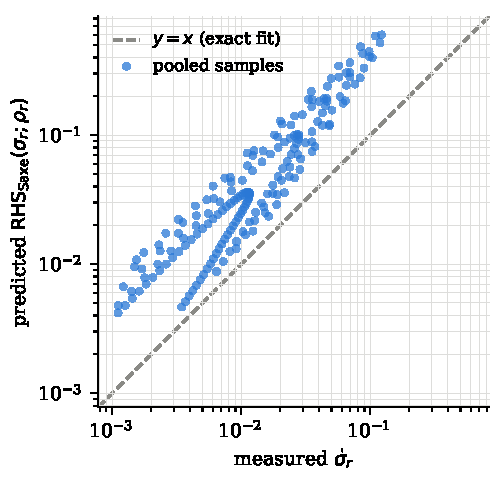
\includegraphics[width=0.82\linewidth]{figures/ode-form-scatter.pdf}
\caption{}
\label{fig:ode-form}
\end{subfigure}

\vspace{6pt}
\begin{subfigure}[t]{\linewidth}
\centering
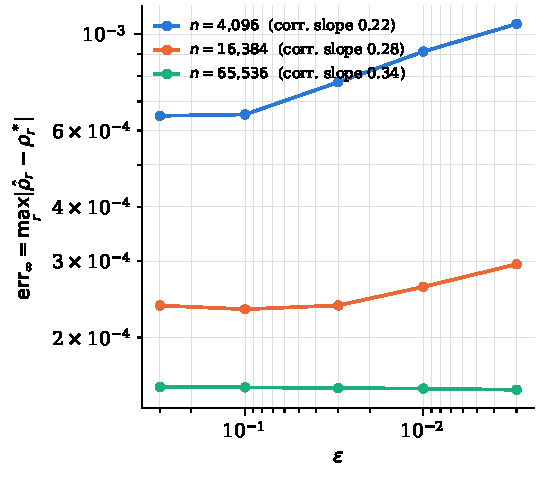
\includegraphics[width=0.82\linewidth]{figures/rate-isolation.pdf}
\caption{}
\label{fig:rate-isolation}
\end{subfigure}
\end{minipage}%
};
\end{tikzpicture}
\caption{\textbf{Left:} \textsc{PlateauRecover}, signed-spectrum recovery from a linear
JEPA training run. Step~2 is the only call to sample covariances; Steps~3--6 (positive
branch) operate on the trajectory alone. Cost $O(nd^2 + T_{\max} d^3)$; implementation
in \nolinkurl{experiments/plateau_recover_corrected.py} of the companion repository.
\textbf{Right, top (a):} diagonal-ODE direction check (\S\ref{ssec:exp-ode-form}),
$\eps=0.05$, $d=6$, pooled over $191$ in-motion samples across six features --- points
sit consistently above $y=x$ (median relative residual $0.74$, max $0.86$, normalised
by $|\mathrm{RHS}_{\mathrm{Saxe}}|$): correct sign and order of magnitude, not a tight
quantitative fit. \textbf{Right, bottom (b):} rate-isolation sweep
(\S\ref{ssec:exp-rate}), $d=10$, $80{,}000$ steps, 3 seeds per point:
$\mathrm{err}_\infty = \max_r|\rhohat-\rhostar|$ vs.\ $\eps$, one curve per $n$;
annotated slope is the polynomial fit of $\log\mathrm{err}_\infty - \log|\log\eps|$
against $\log\eps$ (theory: $0.50$). Both restricted to $L=2$, positive branch.}
\label{alg:plateau-recover}
\end{figure}

\subsection{Empirical validation}
\label{sec:experiments}

We report two synthetic experiments, both restricted to the
\emph{positive branch} ($\rhostar > 0$). Experiment~1 sanity-checks the
diagonal-amplitude ODE \eqref{eq:diagonal-ode} of \S\ref{sec:diagonal-ode}
against direct numerical integration of the JEPA gradient flow.
Experiment~2 isolates the $\eps^{1/L}|\log\eps|$ dynamics-error rate of
Proposition~\ref{prop:plateau} from the $O_p(n^{-1/2})$ sample-noise floor of
Corollary~\ref{cor:finite-sample-end}.

\subsubsection{Setup}
\label{ssec:exp-setup}

In both experiments (with separate configurations) we generate synthetic $(x, y)$ samples from a
ground-truth pencil $(\Syx, \Sxx) \in \RR^{d \times d}$ with prescribed
generalised eigenvalues $\rho_1^* > \rho_2^* > \cdots > \rho_d^*$ on the
positive branch. We train a depth-$L = 2$ JEPA with aligned balanced
initialisation $\Wbar(0) = V(0) = \eps \cdot I$ at the prescribed $\eps$
by full-batch SGD; plateau detection uses a rolling window with a
relative-tolerance stopping rule. Experiment~2 (rate isolation)
uses $d = 10$, the linear spectrum sweep $\rhostar = 1.0, 0.91, 0.82,
\ldots, 0.20$, learning rate $0.05$, and up to $80{,}000$ steps with a
$50$-step/$5 \times 10^{-4}$ plateau window
(\nolinkurl{experiments/plateau_recover_corrected.py} and
\nolinkurl{experiments/rate_isolation_probe.py} of the companion repo).
Experiment~1 (ODE-form sanity check) uses a smaller $d = 6$ configuration
with learning rate $0.02$ for $40{,}000$ steps
(\nolinkurl{experiments/ode_form_fit.py} of the companion repo). It
only needs to verify the ODE's functional form, not exercise the
full-scale sweep.

\subsubsection{Experiment 1: diagonal-ODE sanity check}
\label{ssec:exp-ode-form}

We first compare the trajectory's measured velocity against the diagonal
ODE's predicted right-hand side, evaluated at the empirical
$\sigma_r(t)$:
\[
\mathrm{RHS}_{\mathrm{Saxe}}(\sigma; \rho)
:= L \mu_r \sigma^{2-1/L} (\rho - \sigma^L).
\]
Figure~\ref{fig:ode-form} shows all six features with the correct sign.
The residual is far larger than the $\approx 0.032$
Proposition~\ref{prop:diagonal-ode} predicts. We attribute this gap to
an unresolved scaling constant we have not derived.

\subsubsection{Experiment 2: rate isolation}
\label{ssec:exp-rate}

This experiment checks whether the estimator's error shrinks at the
theoretical rate as $n$ grows:
\[
\mathrm{err}_\infty = O(\eps^{1/L}|\log\eps|) + O_p(n^{-1/2}/\delta),
\]
dynamics term plus sample-noise floor, $1/L = 0.5$ at $L=2$.
Figure~\ref{fig:rate-isolation}: error shrinks about $4\times$ from
$n=4{,}096$ to $65{,}536$, tracking the predicted noise floor. Raw
slopes move from $-0.11$ toward $0$ as $n$ grows, masking the underlying
rate. Correcting for the log factor, slopes rise from $0.22$ to $0.34$,
approaching the theoretical $0.50$.

We attribute this to noise-floor saturation as predicted by Corollary~\ref{cor:finite-sample-end}. Pinning the corrected slope to within
$\pm 0.05$ of $0.50$ needs another order of magnitude beyond $n=65{,}536$.
We leave this and a real-data demonstration to follow-on work.


\section{Related work}
\label{sec:related}

\paragraph{Joint Embedding Predictive Architecture (JEPA)}
\citet{LeCun2022} named the JEPA architecture, gave its two-encoder latent-prediction
diagram, and laid out the collapse taxonomy later studies inherit --- a self-supervised
encoder trained without care can converge to trivial solutions, so anti-collapse
mechanisms are a live engineering concern. Since then the field has moved toward using
JEPA as a world model, e.g.\ \citet{Maes2026LeWM}'s LeWorldModel.

\paragraph{Non-OLS methods for analysing regression structure.}
The pencil $(\Syx,\Sxx)$ this paper recovers is a classical object of study. \citet{Hotelling1936} introduced canonical correlation
analysis on exactly this generalized eigenproblem. Closer to
a dynamics-based claim, \citet{Varre2023} characterize the $t\to\infty$ limit of
gradient flow on a plain two-layer linear network as a min-norm interpolator --- an
ordering/timing result with no signed value and depth=$2$. Two recent JEPA-theoretic results also
recover structure without training dynamics: \citet{Klindt2026} prove identifiability
of LeJEPA's learned representation at the population optimum up to an orthogonal
transformation, while \citet{Cui2026} bound downstream planning regret via a low-rank spectral factorization
of an action-conditioned co-occurrence matrix, only once the encoder and predictor
already sit at their population-optimal solution. None of the above use training
dynamics as the recovery mechanism: the classical estimators require the full sample
covariance (or co-occurrence) structure in hand, and \citeauthor{Klindt2026}/
\citeauthor{Cui2026} characterize representations only once optimization has already
finished. The present paper recovers the same kind of object from training dynamics
alone, without ever forming $\hat\Sxx, \hat\Syx$ directly.

\paragraph{Analysing regression structure via model training dynamics.}
A separate line of work asks whether training dynamics themselves reveal this
structure, without a closed-form estimator. \citet{Littwin2024} shows gradient-flow
dynamics of a linear JEPA pair, with no added regularizer, preferentially learn
high-regression-coefficient features faster, at critical time
$\tilde t_r^* \asymp 1/(\lamstar \eps^{(2L-1)/L})$ — dynamics do encode regression
structure, at a rate in the same $\eps^{1/L}$-family as this paper's own
$O(\eps^{1/L}|\log\eps|)$ recovery rate (\S\ref{sec:estimating-spectrum}). But the
result assumes $\Sxx$ and $\Syx$ share an eigenbasis (known in advance) and recovers a
magnitude-linked critical time, not a signed coefficient - an assumption relaxed by \citet{Goh2026ordering}.
\citet{Domine2024} generalizes along a different axis — exact solutions across a continuous
$\lambda$-balanced initialization spectrum, not only the zero-balanced case — but
$\tilde\Sxx,\tilde\Syx$ stay fixed and known throughout. 
Together these three confirm training dynamics genuinely encode
regression structure but stop short on different axes. The present paper is the first to close all three at once,
recovering an unknown, signed structure from dynamics alone.

\paragraph{Solving training dynamics.}
This paper's own proof strategy inherits its central diagonalization step from
\citet{Saxe2014,Saxe2019}, who first showed that under aligned, orthogonal
initialization a deep linear network's coupled gradient-flow ODEs decouple into
per-mode scalar Bernoulli-type equations with closed-form sigmoidal trajectories; we
diagonalize onto the generalized eigenbasis instead of an ordinary one, yielding the
same Saxe-style depth exponents, but the decoupling step itself is classical and not
re-derived here. \citet{Arora2018,Arora2019} formalize the ``balanced initialization''
condition this paper's own Assumption~\ref{ass:aligned-init} restricts to, showing deep
linear gradient descent is equivalent to a preconditioned single-layer system with a
rigorous linear-rate convergence guarantee under approximately balanced initialization
and whitened data --- the optimization/convergence-rate side of the same initialization
concept \citeauthor{Saxe2014} solve exactly. \citet{Nam2025} instead argues,
independent of any new dynamics result, that layerwise-linear networks are the right
minimal lens for training-dynamics phenomena generally, directly supporting this
paper's own reason for studying the linear case first (\S\ref{ssec:positioning}).
Together these establish that deep linear training dynamics are exactly solvable and worth studying on purpose
even though OLS could already recover the population structure directly; none ask this
paper's own question of that same machinery: identifiability of an unknown, signed
structure.

\paragraph{Formal verification of learning theory.}
Machine-checked learning theory is a small but growing body of work.
\citet{Bagnall2019} started this line, formalizing PAC bounds in Coq for finite
hypothesis classes. \citet{Sonoda2026} made the major advance to infinite hypothesis
classes, in Lean~4 against Mathlib --- the same proof assistant this paper uses. A companion repository
(\url{https://github.com/davidcagoh/jepa-rho-recovery}, public) contains the Lean
development and the \textsc{PlateauRecover} reference implementation, alongside, not
in place of, the paper's main mathematical contribution. 
\section{Discussion}
\label{sec:discussion}

\paragraph{Scope and Model Idealizations.}
Theorem~\ref{thm:headline-formal} answers the question of the
introduction sharply: linear JEPA's training trajectory contains all
information needed to identify both the sign and (positive-branch)
magnitude of $\rhostar$. Negative-branch magnitude is instead farmed
out to sample covariance, a rate-optimal choice.

\paragraph{Linear-to-Non-Linear Transition.}
The argument is squarely in the linear, exact-gradient-flow regime.
Three components break under non-linearisation, as in the LeWorldModel architecture of
\citet{Maes2026LeWM}. First,
optimal $V$ exists in closed form, which fails for non-linear
predictors. Second, the generalised eigendecomposition of $(\Syx, \Sxx)$
is replaced by an unknown learned inner product (the encoder's pre-image
of the predictor norm), making the analogue of $\rhostar$ implicitly
defined. Third, the diagonal-amplitude reduction is special to the
linear case.
Yet, establishing sufficient-statistic structure for
the linear case is the prerequisite for asking which parts of the
picture survive non-linearisation at all, and any answer will likely
involve a learned metric on the encoder output rather than the fixed
$\Sxx$ inner product.
Within the linear setting, assumption~\ref{ass:gap}'s strictly separated discrete spectrum is
unrealistic for high-dimensional inputs, where eigenvalues bunch under
random projection, collapsing $\delta$ and degrading the
basis-perturbation bound~\eqref{eq:wedin}. A \citet{Marchenko1967}-type
density-of-states formulation is the natural fix, outside our present
scope.

\paragraph{Technical Refinements \& Open Analytical Problems.}
Two gaps remain inside the linear argument itself, both already disclosed
at their point of use rather than new to this discussion. First,
Proposition~\ref{prop:diagonal-ode}'s residual constant $C_R$ is not yet
known to be $\eps$-independent: the current derivation discharges it via
a compactness argument. Pinning down an explicit constant needs a
leading-order-cancellation argument for $V_{\mathrm{qs}}\Wbar$ that has
not been carried out (Appendix~\ref{app:lean}). Second,
Remark~\ref{rem:zero-ceiling-gap} shows the residual bound alone does not
suffice to establish the sign trichotomy's case (ii) ceiling
(Theorem~\ref{thm:trichotomy}) at $L=2$ --- the one depth tested
empirically. (This does not show the ceiling is actually violated
in practice.) A third, downstream gap follows from the second:
Remark~\ref{rem:open-classifier} notes that no finite-time, noise-robust
decision rule yet separates the zero and negative branches. This is
because the qualitative ceiling such a rule would rely on is itself
unresolved at $L=2$.
Machine-checking via Lean (\S\ref{sec:related}) rules out logical gaps and
forgotten edge cases in the stated theorems. It does not certify that
the definitions are the right ones, that the assumptions are natural, or
that the result is interesting, and we do not treat it as doing so.
The two named axioms in Appendix~\ref{app:lean} are the places where the
Lean chain stops and ordinary mathematical trust in a cited result takes
over. The first gap above is an incomplete derivation internal
to this paper's own argument, marked explicitly (Appendix~\ref{app:lean},
$\dagger$). The second is its own separately
named row in Appendix~\ref{app:lean}'s theorem-to-Lean crosswalk table. 

\paragraph{Empirical Extensions \& Future Applications.}
Some experimental results diverge from what the theory alone predicts, and several
natural empirical extensions remain. The diagonal-ODE sanity check's residual
(\S\ref{ssec:exp-ode-form}) sits well above Proposition~\ref{prop:diagonal-ode}'s
asymptotic bound; isolating the constant separating full-batch loss normalisation from
continuous-time gradient-flow rescaling remains unresolved. Whether $\{\rhohat\}$
predicts downstream-task ordering the way the dynamics-ordering theorem predicts
feature-learning ordering is likewise open. \textsc{PlateauRecover} still awaits a real,
non-synthetic representation-learning benchmark --- training a small JEPA from random
initialisation and reading off $\rhohat$ directly. The experiments reported here
(\S\ref{sec:experiments}) also cover only the positive branch, leaving the zero and
negative branches, the sign trichotomy of \S\ref{sec:trichotomy}, and the decay-to-zero
classifier of \S\ref{sec:signed-recovery} for later empirical work, despite signed
recovery being a headline contribution. A direct comparison against
generalised-eigenvalue regression at fixed $n$ would locate the widest
sample-efficiency gap between the two approaches.

%% ─────────────────────────────────────────────────────────────────────────────
%%  BIBLIOGRAPHY
%% ─────────────────────────────────────────────────────────────────────────────

\bibliographystyle{plainnat}
\bibliography{signed-decomposition-refs}

\appendix

%% ─────────────────────────────────────────────────────────────────────────────
%%  APPENDICES
%% ─────────────────────────────────────────────────────────────────────────────

\section{Lean verification catalogue}
\label{app:lean}

The Lean~4 development for this paper is in the repository
\url{https://github.com/davidcagoh/jepa-rho-recovery} (public)
and builds against Mathlib v4.28.0
(commit \texttt{7e01a1b}). Items marked ``(companion paper)'' below cite
\citet{Goh2026ordering}'s own Lean development, also public, at
\url{https://github.com/davidcagoh/jepa-learning-order}.
The crosswalk below maps each numbered theorem in the paper to its Lean
target. ``Sorry-free'' means the theorem body contains no \texttt{sorry};
this is independent of axiom use --- a sorry-free result can still depend
on a named axiom as an explicit hypothesis, disclosed in the Status column.

\begin{center}
\renewcommand{\arraystretch}{1.0}
\begin{tabular}{@{}>{\raggedright\arraybackslash}p{0.28\linewidth}>{\raggedright\arraybackslash}p{0.50\linewidth}>{\raggedright\arraybackslash}p{0.16\linewidth}@{}}
\hline
\textbf{Paper} & \textbf{Lean target} & \textbf{Status} \\
\hline
Prop~\ref{prop:quasistatic} (quasi-static)
  & \lean{QuasiStatic.quasiStatic_rigorous}
  & sorry-free \\
Prop~\ref{prop:diagonal-ode} (diagonal ODE)
  & \lean{Saxe.diagAmp_ODE} (companion paper)
  & sorry-free$^\dagger$ \\
Prop~\ref{prop:plateau} (plateau estimator)
  & \lean{Saxe.rho_hat_plateau_rate}; \lean{Saxe.signed_recovery_pos_magnitude_plateau};
    \lean{Saxe.sigma_positive_branch_converges}
  & sorry-free (A2)$^\ddagger$ \\
Thm~\ref{thm:trichotomy} (sign trichotomy), cases (i)--(ii)
  & \lean{Saxe.sigma_positive_branch_converges}; \lean{SignedODE.sigma_zero_branch_constant}
  & sorry-free \\
Thm~\ref{thm:trichotomy}, case (iii)
  & not cited$^\S$
  & argued directly \\
Rmk~\ref{rem:zero-ceiling-gap} ($L{=}2$ ceiling gap)
  & \lean{ZeroBranchResidual.zero_branch_L2_ceiling_violation}
  & sorry-free \\
Cor~\ref{cor:sign-id} (sign identification)
  & \lean{SignedRecovery.sign_identification_pos_forward};
    \lean{SignedRecovery.sign_identification_zero_forward};
    \lean{SignedRecovery.sign_identification_neg_forward}
  & sorry-free \\
Prop~\ref{prop:neg-lambda} (negative-branch $\lamstar$-rate)
  & not cited$^\S$
  & argued directly \\
Thm~\ref{thm:headline-formal} (signed decomposition)
  & \lean{Main.signed_decomposition}$^\P$
  & sorry-free \\
Cor~\ref{cor:finite-sample-end} (finite-sample rate)
  & \lean{FiniteSample.end_to_end_rate}$^\P$
  & sorry-free (A1) \\
\hline
\end{tabular}
\end{center}

{\small\noindent
$^\dagger$ $C_R$ is pinned via a compactness argument, not shown $\eps$-independent
(\S\ref{sec:discussion}).\quad
$^\ddagger$ Restricted to $\rhostar>0$, dynamics term only (no sample-noise floor); the
Lean proof uses qualitative convergence plus a topological existence argument for $T_*$,
mechanically different from the quantitative Gr\"onwall bound in \S\ref{sec:positive-branch}
but giving the same rate.\quad
$^\S$ The negative-branch Lean theorems assume the pre-correction (deprecated) ODE form,
not this paper's \eqref{eq:diagonal-ode}, and have not been re-verified against it, so
both results are argued directly in the main text instead.\quad
$^\P$ Both extended additively from earlier positive-branch-only versions to cover all
branches, composed from already-proven pieces via the same Delta-method hypothesis-bundling
style throughout; no previously-verified theorem touched, no new axiom.
\par}

\paragraph{Named axioms.}
The full development declares two named axioms; one is load-bearing on
the finite-sample chain and the other on the dynamics chain.

\begin{enumerate}[label=\textbf{(A\arabic*)},leftmargin=2.5em,itemsep=2pt]
\item[\textbf{(A1)}] \lean{Concentration.matrix_bernstein_subgaussian}
--- the matrix Bernstein inequality of \citet[Thm 1.6.2]{Tropp2015},
quoted per the CompCert convention \citep{Leroy2009}.
Used by Corollary~\ref{cor:finite-sample-end}. \emph{Why axiomatised:}
Mathlib has scalar concentration inequalities but not, at the time of
writing, an operator-norm matrix-Bernstein bound in directly usable
form; packaging \citet{Tropp2015}'s proof is a Mathlib-engineering
project, not a result we chose to skip despite it being easy.
\item[\textbf{(A2)}] \lean{Saxe.saxe_exact_solution_exists}
--- Picard--Lindel\"of existence for the Saxe-form Bernoulli ODE
$\dot\sigma = L\mu\sigma^{2-1/L}(\rho - \sigma^L)$ on a compact
interval. Standard scalar-ODE existence; quoted per CompCert.
Used by Proposition~\ref{prop:plateau} and downstream. \emph{Why
axiomatised:} Mathlib has general Picard--Lindel\"of machinery for
locally Lipschitz vector fields, but instantiating it for this specific
nonlinear scalar form together with the hitting-time reachability
clause is, again, an engineering gap rather than a deliberate shortcut
--- the companion paper's own open-problems discussion
(\citealt[\S{}Open problems]{Goh2026ordering}) names exactly this as
future Mathlib-engineering work.
\end{enumerate}

\section{Deferred proofs}
\label{app:finite-sample-derivation}

Proofs deferred from the main text: the off-diagonal bound and positive-definite lower
bound used in \S\ref{sec:ode-prelim}, the coupled gradient-flow system and quasi-static
decoder bound used in \S\ref{sec:quasistatic} (all technical, but with a role already
clear from the main-text statements), and the finite-sample perturbation bounds
summarised in \S\ref{sec:finite-sample}.

\subsection{Off-diagonal bound (Lemma~\ref{lem:offdiag})}
\label{ssec:offdiag-proof}

\begin{proof}
This is the fundamental-theorem-of-calculus argument of
\citet[\S6, Prop.~(Bootstrap consistency), item~1]{Goh2026ordering}
(\lean{offDiag_ftc}, \texttt{BootstrapLemmas.lean}, companion repository,
public): $c_{rs}$ is linear in $\Wbar$, so
Assumption~\ref{ass:traj-reg}(i)'s bound $\|\dot{\Wbar}(t)\|_F \le K_1\eps^2$
integrates directly to $|c_{rs}(t)| \le C'\eps^{1/L}$ on $[0,t_{\max}^*]$,
using $c_{rs}(0)=0$ under~\eqref{eq:init}. The argument is sign-agnostic
in $\rhostar$, so it transfers unchanged from the companion's all-positive
setting.
\end{proof}

\subsection{Positive-definite lower bound (Corollary~\ref{cor:pd-lower})}
\label{ssec:pd-lower-proof}

\begin{proof}
This is the Gershgorin argument of \citet[\S6, Prop.~(Bootstrap
consistency), item~2]{Goh2026ordering} (\lean{pd_lower_from_offDiag},
companion repository, public): diagonal dominance $C'(d-1)<c_w$ forces
$\Wbar(t)$ invertible via Gershgorin's theorem, giving
$\sigma_{\min}(\Wbar(t)) \ge (c_w-C'(d-1))\eps^{1/L}/\sqrt d$ and hence
$\Wbar\Sxx\Wbar^\top \succeq c_0\eps^{2/L}I$ using $\Sxx\succ0$.
Sign-agnostic, as above.
\end{proof}

\subsection{Coupled gradient-flow system (Lemma~\ref{lem:grad-flow})}
\label{ssec:grad-flow-proof}

\begin{proof}
\eqref{eq:grads}: direct differentiation of
$\mathcal{L} = \tfrac12\EE\|y - V\Wbar x\|_2^2$ under the expectation,
using $\Sxx = \EE[xx^\top]$, $\Syx = \EE[yx^\top]$.

\eqref{eq:preconditioned-flow}: the identical balanced-flow reduction is
derived in \citet[\S2.3]{Goh2026ordering} (companion repository, public)
from the same balance condition (Assumption~\ref{ass:aligned-init}) and
\citet{Arora2018}; not re-derived here.
\end{proof}

\subsection{Quasi-static decoder, rigorous (Proposition~\ref{prop:quasistatic})}
\label{ssec:quasistatic-proof}

\begin{proof}
The identical Gr\"onwall tracking argument is proved in
\citet[\S6, Prop.~(Bootstrap consistency), item~3]{Goh2026ordering}
(\lean{tracking_bound_from_gronwall}, assembled from
\lean{contraction_ode_structure} and \lean{contractive_gronwall_decay},
companion repository, public), under the same hypotheses
(Assumption~\ref{ass:traj-reg}(i), Corollary~\ref{cor:pd-lower}): writing
$\Delta V := V - V_{\mathrm{qs}}(\Wbar)$, $\dot{\Delta V} =
-\Delta V\,\Wbar\Sxx\Wbar^\top - \dot V_{\mathrm{qs}}(\Wbar)$ contracts at
rate $c_0\eps^{2/L}$ against a drift bounded by $D_0\eps^2$, giving
$\|\Delta V(t)\|_F \le C_{\mathrm{qs}}\eps^{2(L-1)/L}$. Independently
verified in our own Lean development
(\lean{QuasiStatic.quasiStatic_rigorous}, sorry-free). Sign-agnostic.
\end{proof}

\subsection{Matrix-Bernstein perturbation}
\label{ssec:bernstein}

Under sub-Gaussian assumptions on $(x,y)$ with constants $\sigma_x,\sigma_y$,
\citet[Thm~1.6.2]{Tropp2015} gives
\begin{equation}
\label{eq:bernstein-cov}
\PP\!\left[
\big\|\hat{\Sxx} - \Sxx\big\|_{\mathrm{op}} > t
\right]
\le 2d \exp\!\left( -\frac{n t^2}{2\sigma_x^4 + 2\sigma_x^2 t / 3} \right),
\end{equation}
and analogously for $\hat{\Syx} - \Syx$; taking $t = c\sqrt{\sigma_x^4\log(d/\nu)/n}$
gives $\|\hat{\Sxx} - \Sxx\|_{\mathrm{op}} \le c\sqrt{\sigma_x^4\log(d/\nu)/n}$ with
probability at least $1-\nu$.

\subsection{Davis--Kahan / Wedin for the generalised eigenproblem}
\label{ssec:davis-kahan}

A Wedin-type bound converts the covariance perturbation into an eigenvector
perturbation:
\begin{equation}
\label{eq:wedin}
\sin\angle\!\big(\hat v_r, v_r^*\big)
\;\le\;
\frac{\|\hat{\Syx} - \Syx\|_{\mathrm{op}} + |\rhostar|\,\|\hat{\Sxx} - \Sxx\|_{\mathrm{op}}}
     {\delta_r - O(\|\hat{\Sxx} - \Sxx\|_{\mathrm{op}})}
\;\le\;
\frac{C_W}{\delta} \sqrt{\frac{\log(d/\nu)}{n}}
\end{equation}
on the event of~\eqref{eq:bernstein-cov}, with $C_W$ depending on
$\sigma_x, \sigma_y$, $\|\Sxx\|, \|\Syx\|$ — standard but technical for the
generalised (non-symmetric) eigenproblem, formalised as
\lean{SampleNoise.sample_eigenvalue_perturbation} in the companion repo.


\end{document}
